\documentclass[12pt]{article}
\setlength{\textwidth}{17cm}
\setlength{\textheight}{24cm}
\setlength{\topmargin}{-2cm}
\setlength{\footskip}{1cm}
\setlength{\evensidemargin}{0cm}
\setlength{\oddsidemargin}{0cm}
\setlength{\parindent}{0.75cm}

\usepackage{allrunes}
\usepackage{amsmath}
\usepackage[magyar]{babel}
\usepackage[T1]{fontenc}
\usepackage[utf8]{inputenc}
\usepackage{fixltx2e}
\usepackage{multirow}

\usepackage[hyphens]{url}
\usepackage[unicode,colorlinks=true,breaklinks]{hyperref}
%\usepackage[dvips]{hyperref}
%should display links, but it does not work with \H accent
%and formulas in section titles

\hypersetup{colorlinks,linkcolor=blue,urlcolor=magenta,citecolor=magenta}
%Breaks long url`s in text, while keeping it one link:

\usepackage{amsfonts}
\usepackage{amsthm}
\usepackage{amssymb}


\theoremstyle{plain}
\usepackage{graphicx}

%\usepackage{gensymb}
\usepackage{float}

% For bra-ket notation
\usepackage{braket}

%% New commands
\newcommand{\dd}{\textrm{d}}



\begin{document}
\title{15. tétel \\ Relációs adatbázisok}
\author{Bulatovic Nikola}

\maketitle

\begin{abstract}
     A relációs adatmodell, logikai és fizikai operátorok (seek, scan és a joinok változatai, aggregálás), adattárolási modellek (row store, column store), indexek (klaszterezett index, nem klaszterezett index), a B-fa, kulcsok és kényszerek, tranzakciók. Lekérdezésoptimalizálás. Az adatbetöltés menete. \par
     Ez a tétel az \textit{Adatmodellek és adatbázisok a tudományban} kurzus alapján készült \cite{db}. Megjegyzés: az utolsó fejezetek témakörei (Tranzakciók kezelése c. fejezettől) csak említés szintjén szerepeltek az előadáson, így ezek nincsenek részletesen kidolgozva.
\end{abstract}

\tableofcontents
\newpage


\section{Bevezetés - adatbázis szerverek}

Az adatbázis szerver általában olyan dedikált szerver, amely különféle adatbázis szolgáltatásokat nyújt más gépeknek vagy programoknak a kliens-szerver modell alapján leírt módokon. Az ilyen szervereken a háttértár, az I/O és a hálózat konfigurációja erősen optimalizált. Az adatbázis szerver fő feladatai:
\begin{itemize}
    \item rendezett adattárolás a megmaradó (non-volatile) memóriában vagyis a háttértárolón
    \item lekérdezések (query) gyors végrehajtása
    \item adatmódosítás
    \item tranzakciók kezelése (hosszú, konkurens műveletek atomizált végrehajtása)
    \item adat konzisztencia fenntartása
    \item adatbiztonság (rendszerhiba esetén is megmaradó adatok)
\end{itemize}{}
Többféle adatbázis kezelő rendszer (database management system - DBMS) létezik, melyek ilyen adatbázis szerver funkcionalitással rendelkeznek. Az egyik legismertebb és legtöbbet használt a relációs adatbázis kezelő rendszerek (RDBMS). Ezeknek többféle implementációja létezik: Oracle, Microsoft SQL Server, vagy a nyílt forráskódú Postgres és MySQL. Ezek közös tulajdonsága, hogy mindegyik relációs adatmodellt alkalmaz, a lekérdezésekhez pedig egy adat-orientált deklaratív nyelvet az SQL-t (Structured Query Language) használ. 


\section{Relációs adatmodell}

Az adatbázisok logikai alapeleme a tábla (table). A táblák oszlopait a séma jellemzi: az adattípus és méret előre definiált. Az adatot magát a tábla sorai jelentik, amelyek száma tetszőleges és azonos formátumúak. A táblákon belül különböző megkötések (contrains) lehetnek: 
\begin{itemize}
    \item[-]elsődleges kulcs (primary key), ami a táblán belül egyedi, és egy vagy több oszlop kombinációja, mellyel a rendezés jól definiált (kulcsok összehasonlíthatóak <,>,=) 
    \item[-]másodlagos kulcs (foreign key), ami egy másik tábla elsődleges kulcsára mutat
\end{itemize}{}
Az adatbázisok működési logikáját a relációs adatmodell írja le, melynek matematikai alapja a relációs algebra. A relációs adatszerkezet alapfogalmai a következők:
\begin{itemize}
    \item \textbf{halmaz}: egy táblázat oszlopa, vagy oszlopok rendezett listája (tuple)
    \item \textbf{műveletek}: Descartes-szorzat, szelekció, projekció, unió, különbség
    \item \textbf{séma}: megkötés, hogy milyen halmazok, milyen sorrendben szorozhatóak össze
    \item \textbf{reláció}: Descartes-szorzat részhalmaza.
\end{itemize}{}
A logikai működést - matematikai precizitás mellőzve- úgy lehet összefoglalni, hogy a lekérdezések a táblázatok Descartes-szorzatán végzett műveletek utáni részhalmaz képzést jelent (\ref{fig:rel}. ábra).


\begin{figure}[H]
    \begin{center}
    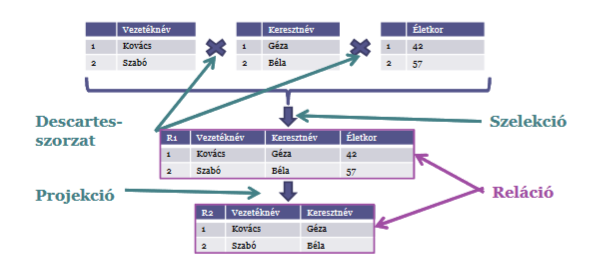
\includegraphics[width=0.85\textwidth]{media/rel.png}
    \caption{\textbf{A relációs algebra sematikus ábrázolása.} A lekérdezés végeredménye (reláció) a halmazok Descartes-szorzatának egy részhalmaza.} 
    \label{fig:rel}
    \end{center}
\end{figure}


\section{Adatok fizikai tárolása az adatbázis szerveren}

Az adatbázisok alapproblémai a következők:
\begin{itemize}
    \item[-] a háttértár mindig jóval lassabb, mint a központi memória és a CPU (megoldás: indexelés)
    \item[-] a háttértár szekvenciálisan sokkal gyorsabban olvasható, mint random módon
    (megoldás: sorok lapokba (page) szervezése, lapok megfelelő sorrendben tárolása)
    \item[-] a memória mérete mindig sokkal kisebb, mint az adatbázis mérete (megoldás: ügyes algoritmusok, hogy ne kelljen transzformálni a memória és a diszken levő formátum között). 
\end{itemize}{}
Az adatok fizikai szervezésének megértése elengedhetetlen ahhoz, hogy lássuk hogyan kell a háttértárat és az adatbázist optimálisan konfigurálni. Sokszoros sebességnövekedés érhető el a naiv adatbázis szervezéshez képest.
\\
\subsection{Lapok}
A fizikai egységek a következők: adatbázis > file group > file > extent > page, illetve a tranzakciós napló. A tárolás alapegysége tehát a lap (\ref{fig:lap}. ábra):
\begin{itemize}
    \item[-] mérete fix 8kB
    \item[-] 8 lap alkot egy extent-et (64 kB)
    \item[-] csak teljes extent írható/olvasható a lemezre/ről
    \item[-] formátum a memóriában és a lemezen azonos
    \item[-] több fajtája van (tábla adat, index stb.)
\end{itemize}{}

\begin{figure}[H]
    \begin{center}
    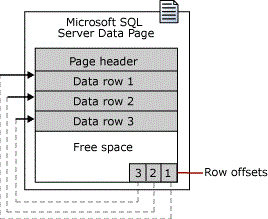
\includegraphics[width=0.55\textwidth]{media/page.png}
    \caption{\textbf{A tárolás alapegysége, a lap (page).} Az adatbázisban tárolt fájlok által allokált tárhely logikailag ilyen lapokra vannak osztva. Minden lap rendelkezik egy headerrel, amely tartalmazza a lap számát, típusát, a maradék üres hely méretét. A táblázat sorai a lapokon tárolódnak sorfolytonosan. Minden lap rendelkezik egy row offset táblázattal, ami megadja hogy a lapon szereplő sorok hányadik bájtnál kezdődnek a lap elejéhez képest.} 
    \label{fig:lap}
    \end{center}
\end{figure}

\subsection{Adatstruktúrák}
Ahogy korábban láttuk az adattárolás logikai egysége a tábla, azon belül pedig a sor. Ha egy tábla sorai nem meghatározott sorrendben tárolódnak (heap table), akkor egy új sor beírása könnyű (az utolsó lap végére kell írni), azonban kereséskor az egész táblát végig kell olvasni. Mint láttuk, az elsődleges kulcs használata egy lehetséges rendezést definiál a sorok között. Ha létezik egy ilyen rendezés, akkor táblát klaszterezett indexszel tárolhatjuk fizikailag.\par
Sorba rendezett adatok tárolására egy lehetséges adatstruktúra a B-fa, amely a hagyományos bináris-fa általánosítása. A bináris fa esetében egy új adatpont beírásakor gyakran az egész fát újra kell építeni, ami használhatatlanná teszi adatok diszken történő tárolására. A B-fa is csomópontokból áll, de az $d$ számú adatsort és $d+1$ számú pointert tartalmaz (bináris esetben $d = 1$). A pointerek további csomópontokra mutatnak, amelyekben található érték a pointer csomópontjában lévő adatok értékei közé esik (\ref{fig:tree}. ábra).

\begin{figure}[H]
    \begin{center}
    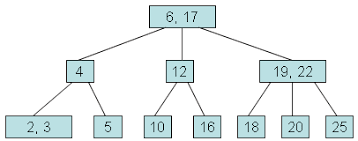
\includegraphics[width=0.65\textwidth]{media/btree.png}
    \caption{\textbf{A B-fa legegyszerűbb sematikus ábrázolása.}} 
    \label{fig:tree}
    \end{center}
\end{figure}

A B-fa építésekor ha egy csomópont betelik, akkor kettéosztjuk. Az ilyen módon konstruált fa egy ún. \textit{self balancing} kereső fa, ami azt jelenti hogy egy elem megtalálása (a fa mélysége) $\sim o(log_dn)$. A B-fa ezzel megoldja a bináris fa problémáit.
\par
Ennek ellenére néhány művelet a B-fa esetében is költséges lehet, a keresett csomópont mélységének függvényében. Ezt a problémát oldja fel a B-fa egy optimalizálása, a B+-fa. Ahelyett, hogy minden csomópontot egyformán kezelne, két típusba sorolja őket: a közbenső szinteken csak a kulcsokat és a pointereket tárolja, a tényleges adatokat csak a legalsó szinten. 
\\
Az adatbázis ilyen B+-fa struktúrában tárolja a táblákat. A fa szintje egy lapnak felel meg. Mivel a B+-fa struktúrában kétféle csomópont van, ezért két fajta lapra van szükség: index és sorokat tároló lap. A lapokon a pointerek a soron következő/előző lapokra mutat (\ref{fig:idx}. ábra). Ez a következő előnyökkel jár: 
\begin{itemize}
    \item[-] a tábla szekvenciálisan, a kulcs szerinti sorrendben (vagy visszafele) olvasható \\
    SELECT * FROM t WHERE id BETWEEN 12 AND 66
    \item[-] egy adott kulcsú sor gyorsan megtalálható \\SELECT * FROM t WHERE id = 12
    \item[-] egy adott kulcs tartomány gyorsan megtalálható, nem kell rendezni \\
    SELECT * FROM t ORDER BY id (ORDER BY elhagyható)
\end{itemize}{}

\section{Indexek}

\subsection{Nem klaszterezett indexek}
Ahogy az előzőekben láttuk egy táblához klaszterezett index építhető, amely jelentősen gyorsíthatja a lekérdezéseket. Egy táblán csak egy ilyen index lehet, amely meghatározza a tárolás sorrendjét. Az optimalizált lekérdezés csak az indexhez tartozó elsődleges kulcs alapján lehetséges. Ha más oszlop szerint is hasonló gyorsasággal szeretnénk keresni, akkor nem klaszterezett indexeket kell használunk.
\par
A nem klaszterezett index a tábla soraitól eltérő struktúrával rendelkezik, mivel az indexek sorrendje nem tükrözi az adatok fizikailag tárolt sorrendjét. Ehelyett az elsődleges kulcstól eltérő oszlop vagy oszlopokra épül és az ezek szerinti sorrendet indexeli. Ezek tárolási struktúrája hasonlóan B+-tree, azonban a fa utolsó (leaf) csomópontjai nem a tényleges adatot tárolják, hanem csak egy arra mutató pointert (\ref{fig:idx}. ábra).

\begin{figure}[H]
    \begin{center}
    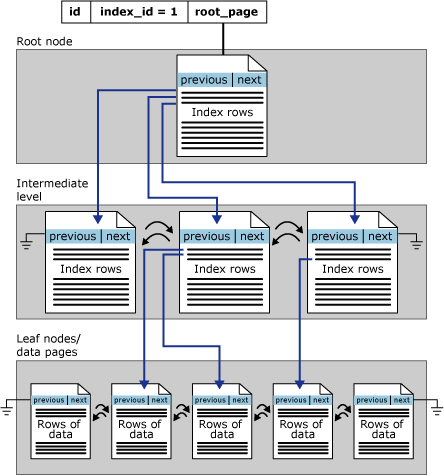
\includegraphics[width=0.45\textwidth]{media/cluster.png}
    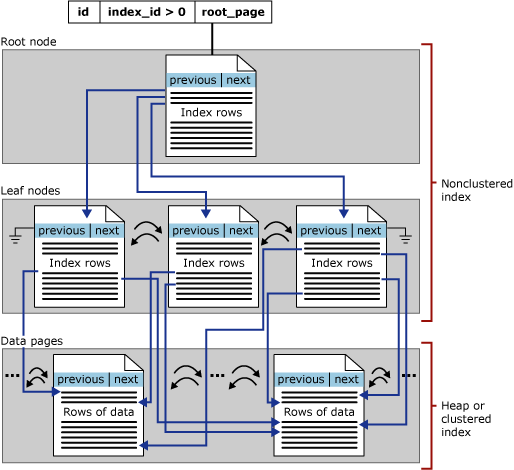
\includegraphics[width=0.5\textwidth]{media/noncluster.png}
    \caption{\textbf{Klaszterezett (bal) és nem klaszterezett index (jobb).} A klaszterezett index esetében a fa levelei a tényleges adatot tárolják. A nem klaszterezett index esetében pedig egy pointer található arra az adat page-re, amelyen a tényleges adat található. Ha a tábla nem rendelkezik klaszterezett indexszel, akkor a pointer heap page-re mutat, ahol az adat van.} 
    \label{fig:idx}
    \end{center}
\end{figure}

\subsection{Beágyazott oszlopok}

Ha olyan lekérdezést írunk, amihez csak az indexelt oszlopok kellenek, akkor elég csak az index struktúrát végigolvasni, az eredmény ezekből egyértelmű. Ha más oszlop is szerepel a lekérdezésben, akkor ezeket külön be kell tölteni a táblából.\par
Nem klaszterezett indexek létrehozásakor hozzáadhatunk beágyazott oszlopokat (included columns) az indexhez olyan formában, hogy az index pointerei mellé bekerülnek ezek az oszlopok is. Ekkor nem kell az adatsort külön betölteni kereséskor.

\subsection{Indexek tulajdonságai}

Indexek használatának előnyei:
\begin{itemize}
    \item[-]adott oszlopok szerinti keresés gyors, de csak ha a legelső indexelt oszlopra erős a megszorítás
    \item[-]az indexelt adatok az előírt sorrendben, szekvenciálisan olvashatóak.
\end{itemize}{}
Hátrányai:
\begin{itemize}
    \item[-]több tárhelyet igényel (az indexelt oszlopok még egyszer tárolódnak)
    \item[-]beszúráskor, módosításkor, törléskor frissíteni kell
\end{itemize}{}


\section{Logikai és fizikai operátorok}

\subsection{Alapvető fizikai operátorok}

\begin{itemize}

    \item \textbf{table scan}: 
        \begin{itemize}
            \item[-] adott index nélküli heap tábla
            \item[-] csak szekvenciálisan olvasható
            \item[-] nincs jól definiált sorrend
            \item[-] query: SELECT * from t WHERE a = 2
        \end{itemize}{}
    
    \item \textbf{sort}: 
        \begin{itemize}
            \item[-] hasonló feltételek mellet, mint a table scannél
            \item[-] query: SELECT * from t ORDER BY a
        \end{itemize}{}
        
    \item \textbf{(clustered) index scan}:
        \begin{itemize}
            \item[-] adott egy t tábla, rajta c indexszel
            \item[-] query-k: SELECT c FROM t WHERE c BETWEEN 5 AND 1 \\ SELECT c FROM t ORDER BY c 
            \item[-] az index eleve definiálja a sorrendet (nem kell sort), más oszlop szerinti sorrend esetén viszont újra kell
            \item[-] klaszterezett indexnél rögtön rendelkezésre áll a többi oszlop
            \item[-] nem klaszterezett indexnél (ha csak a c oszlopra van szükség) elég az indexet olvasni, a táblához nem is kell nyúlni
        \end{itemize}{}
        
    \item \textbf{(clustered) index seek}:
        \begin{itemize}
            \item[-] adott egy t tábla, rajta c egyedi (unique) indexszel
            \item[-] query: SELECT c FROM t WHERE c = 10
            \item[-] egyetlen sor megtalálása $o(log(n))$
            \item[-] ha c nem egyedi, akkor seek helyett scan ($o(n)$)
            \item[-] ezért elsősorban kulcsot esetében használt
        \end{itemize}{}
        
    \item \textbf{bookmark (key) lookup}:
        \begin{itemize}
            \item[-] adott egy t tábla, rajta c nem klaszterezett index
            \item[-] nem csak a c oszlopra van szükség
            \item[-] query: SELECT * FROM t WHERE c BETWEEN 2 AND 10
            \item[-] a sorokat index alapján gyorsan megtaláljuk
            \item[-] az index csak pointereket tartalmaz
            \item[-] pointer (bookmark) alapján kell előszedni a többi oszlopot is (pointer alatt az elsődleges kulcs értendő, heap tábla esetén pedig a rowid)
            \item[-] a random I/O miatt drága művelet
        \end{itemize}{}
        
\end{itemize}{}
\subsection{Logikai join műveletek}

Relációs algebra szerint a join egyszerűen a Descartes-szorzat valamilyen részhalmaza (vagyis egy reláció). Fajtái:

\begin{itemize}
    \item[-] \textbf{cross join}: a teljes Descrates-szorzat: \\
    SELECT * FROM t1 CROSS JOIN t2
    \item[-] \textbf{inner join}: csak az $f()$ feltételnek megfelelő sorok: \\ 
    SELECT * FROM t1 INNER JOIN t2 ON f(t1.c1, t2.c2) 
    \item[-] \textbf{left/right/full outer join}: a bal (t1) vagy a jobb (t2), vagy mindkét táblából azokat a sorokat is hozzáveszi, amikre az f() feltétel soha nem teljesül \\
    SELECT * FROM t1 LEFT OUTER JOIN t2 ON f(t1.c1, t2.c2)
    \item[-] \textbf{semi/anti join}: csak az érdekel, hogy a másik táblában van-e megfelelő (vagy nincs), oszlopok értékeire nincs szükség \\
    SELECT * FROM t1 WHERE t1.ID IN (SELECT t1.ID FROM t2)
    \item[-] \textbf{range join}: ha nem a kulcs konkrét értékeire, hanem egy intervallumra szűrünk \\
    SELECT * FROM t1 INNER JOIN t2 ON t1.ID BETWEEN t2.start AND t2.end
\end{itemize}{}
\bigskip
Az adatbázis három különböző algoritmussal tud join műveletet végrehajtani:
\begin{itemize}
    \item \textbf{nested loop join}:
    \begin{itemize}
        \item[-] ha a táblák nincsenek sorba rendezve, akkor egymásba ágyazott ciklusokkal megy a join
        \item[-] adott a t1 és t2 tábla, c1 illetve c2 oszloppal
        \item[-] query: SELECT *FROM t1 INNER JOIN t2 ON t1.c1 = t2.c2  
        \item[-] külső ciklus egy táblát olvassa, belső ciklus a másikat
        \item[-] ha nincsen megfelelő index, akkor a belső ciklus annyiszor lefut (és beolvassa az adatot a lemezről), ahány sora a külső táblának van
    \end{itemize}{}
    \item \textbf{merge join}:
    \begin{itemize}
        \item[-] ha a join feltétel t1.c1 = t2.c2
        \item[-] a bemeneti tábláknak rendezettnek kell lenniük
        \item[-] a két táblát azonos sorrendben, párhuzamosan, szekvenciálisan olvassa
        \item[-] a lehetséges párok egyszerűen meghatározhatóak
    \end{itemize}{}
    
    \item \textbf{hash match join}:
    \begin{itemize}
        \item[-] az egyik bemeneti táblából hash táblát épít, és az alapján ellenőrzi a másik tábla sorait
        \item[-] adott t1 tábla egy c1 kulccsal és egy elég kicsi tábla c2-vel
        \item[-] c2 értékeire számolható hash, soraiból hash tábla építhető
        \item[-] a join végrehajtásakor t1-et a kulcs szerint olvassuk, a hash tábla pedig megadja ($o(1)$ időben), hogy t2-ben van-e megfelelő sor. Ha van, akkor az a hash táblában van.
    \end{itemize}{}
\end{itemize}{}

\subsection{Aggregátumok}

Az adatbázisban az adatok különböző aggregált mennyiségei is meghatározhatók. A csoportokat a GROUP BY kifejezéssel hozhatunk létre egy vagy több oszlop egyedi értékeiből,
mint például a következő lekérdezésben:
\\
\\
SELECT c1,c2,MIN(c1),count(c2) \\
FROM t \\
GROUP BY c1,c2 \\
HAVING max(c1) > 5 \\
\\
Itt a c1 és c2 oszlop alapján hozunk létre csoportokat. Ezeken a csoportokon különböző
aggregátum függvényeket használhatunk, ami az adott csoport statisztikáját adja meg. Itt
a MIN és a COUNT szerepel, de az összes hasonló jellegű művelet alapértelmezett (MAX, AVG, SUM, stb.).
Ebben a lekérdezésben azokra a csoportokra szűkített a keresés, ahol a csoport c1 oszlopának maximális értéke nagyobb
mint 5.
A beépített függvények mellett lehetőség van felhasználó által definiált aggregátumok létrehozására.
Ekkor három függvényt kell implementálni:
\begin{itemize}
\item[-] accumulate: a következő sort dolgozza fel
\item[-] merge: két részszámolást von össze
\item[-] terminate: a végső számolást végzi el.
\end{itemize} 


\section{Lekérdezésoptimalizálás}


Az SQL deklaratív nyelv: azt fogalmazzuk meg benne, hogy mit szeretnénk eredménynek, nem pedig azt, hogy hogyan számolja ki azt, ezért felmerül a legkérdezések optimalizálásának kérdése. Ez szerver és felhasználói oldalon is fennáll.\par
A szerver a rendelkezésére álló információk (query, indexek, adatbázis séma, hardver) megpróbálja optimalizálni a lekérdezést. Ehhez 
a lehetséges fizikai műveletek sokaságát implementálja: azonos végeredményű, de különböző végrehajtási terveket készít, majd ezek közül megpróbálja kiválasztani azt, aminek a legrövidebb a várható futási ideje.\par

A szerver lehetőségei korlátozottak a rendelkezésre álló információ végessége miatt, ezért a felhasználókra hárul a további optimalizálási
feladat. A felhasználó segítheti a szervert például a fizikai operátorok explicit előírásával, vagy olyan indexek tervezésével, amelyek gyorsítják az összes lehetséges lekérdezés futási idejét. A helyes indexek kiválasztásához a következőket kell figyelembe venni:
\begin{itemize}
\item[-] tartalmazza az összes oszlopot, ami a lekérdezés végrehajtásához kell (beágyazott oszlopok!)
\item[-] megfelelő sorrendben legyen rendezve
\item[-] a lehető legkisebb legyen a lehetséges indexek közül
\end{itemize} 


\section{Tranzakciók kezelése}

A tranzakció több lépésből álló, adatmódosító művelet, melyből több is futhat egyszerre. Az alábbi tulajdonságokkal rendelkezik:
\begin{itemize}
    \item \textbf{atomicity}: a tranzakciók vagy teljes egészében lefutnak, vagy egyáltalán nem okoznak változást
    \item \textbf{consistency}: az adatbázist a tranzakció konzisztens állapotból konzisztensbe viszi
    \item \textbf{isolation}: a párhuzamos tranzakciók csak kontrolláltan interferálhatnak
    \item \textbf{durability}: ha egy tranzakció készre lett jelentve, akkor az többet nem vonható vissza.
\end{itemize}{}
Legegyszerűbb példa tranzakcióra egy bankszámla terhelése egy másik javára. Ez egyben példa a tranzakciók kezelésének problémáira is: először ellenőrizni kell, hogy van-e elég fedezet a bankszámlán. Eközben valaki más terhelheti ugyanazt a számlát, így a tranzakciónak három kimenetele lehetséges: commit (érvényes), rollback (érvénytelen), abort (ütközés).
Az ilyen problémák az tranzakciók izolálásával oldhatók meg, melynek célja a konkurens műveletek párhuzamos futtatása úgy, hogy az adatok konzisztensek maradjanak. Ennek két fő megvalósítása lehetséges: adatok zárolása (lock), adatok verziószámmal történő ellátása.


\section{Az adatbetöltés menete}

Az adatok betöltésére három mód lehetséges:
\begin{itemize}
    \item INSERT utasítások (nem effektív, rossz megoldás)
    \item kliens könyvtár használata (közepesen jó megoldás)
    \item BULK INSERT (legjobb megoldás, nagy mennyiségű adat betöltésére optimalizált)
\end{itemize}{}

Az adatbetöltés bevált gyakorlatai:
\begin{itemize}
    \item Vizuális eszközök helyett scriptek (source control alá vonható, megjegyzésekkel látható el, metaadatokat is tartalmazhat)
    \item text formátum előnye (bináris forrásfájl helyett érdemes szöveges fájlokat használni a bulk inserthez, mert kezdetben sokkal könnyebb megtalálni a hibákat)
    \item betöltés kisebb mennyiségekben (ha valami elromlik betöltés közben, sokkal könnyebb a hibát megtalálni és a betöltést megismételni)
    \item indexek tesztelése építés előtt
    \item idegen kulcsok tesztelése
\end{itemize}{}


\section{Oszlopalapú adattárolás}
Az eddigiekben a sor alapú tárolási modellről esett szó. Ez a módszer főleg tranzakciók kezelését végző adatbázis esetében optimális. Ezzel a fő probléma, hogy a sorfolytonos tárolás miatt sok olyan adatot (oszlopot) be kell olvasni, ami nem szerepel a lekérdezésben. \par
Ezt a problémát oldja fel többek között az oszlop alapú tárolási mód. Ez egy új technológia, amivel jobb teljesítmény érhető el olyan adatoknál, amik nem változnak. Oszlop alapú tárolás esetében a relációs algebra alapjai is megváltozik: a logikai egység (tábla) nem sorok, hanem oszlopok összessége. Ebből adódóan az összes logikai művelet (pl.: join) is megváltozik. A módszer hátránya, hogy a sajátos logikából adódóan az adatok módosítása nagyon költséges művelet, így ez a módszer sem használható univerzálisan. Egy modern és jól működő adatbázisban vannak sor- és oszlopalapú táblák is.


\bibliographystyle{plain}
\bibliography{references}

\end{document}
